\documentclass[aspectratio=169]{beamer}
\usetheme[pattern=network,color=nudarkblue,numbering=progressbar,sectionpage=none,agendastyle=plain]{wildcat}
\usepackage[french]{babel}
\usepackage{booktabs,tabularx}
\newcolumntype{L}[1]{>{\raggedright\arraybackslash}p{#1}}
\renewcommand{\tabularxcolumn}[1]{>{\raggedright\arraybackslash}p{#1}}
\pdfstringdefDisableCommands{\def\\{ }}
\title[Approche agentique et trading multifactoriel]{L'approche agentique dans un\\contexte de trading multifactoriel}
\subtitle{Prototype supervisé et évaluation d'une synthèse LLM}
\author[SANOU Abou Dramane]{SANOU Abou Dramane\\Master Finance de marché · CNAM\\Encadrant : Bertrand DJEMBISSI}
\date{Septembre 2026}
\titlegraphic{\includegraphics[height=1.15cm]{assets/logo\_cnam.png}}
\newcommand{\source}[1]{\par\vfill{\tiny\color{black!60}Source : #1\par}}
\newcommand{\takeaway}[1]{\par\vspace{0.5em}{\color{wcprimary}\textbf{#1}\par}}
\newcommand{\oral}[2]{\note{#1\par\medskip [Sources] #2 [/Sources]}}
\setlength{\emergencystretch}{1em}
\ifdefined\notesonly\setbeameroption{show only notes}\fi
% Couverture du thème adaptée pour afficher le sous-titre et l'encadrant.
\setbeamertemplate{title page}{%
  \vspace*{2.0cm}
  {\usebeamerfont{title}\color{white}\inserttitle\par}
  \vspace{0.25cm}
  {\small\color{white}\insertsubtitle\par}
  \vspace{0.45cm}
  {\usebeamerfont{author}\color{white}\insertauthor\par}
  \vspace{0.2cm}
  {\usebeamerfont{author}\color{white}\insertdate\par}
}
\begin{document}
\begin{frame}
  \titlepage
  \oral{30 s. Présenter le sujet : étudier comment un agent peut restituer des résultats financiers calculés ailleurs. La contribution porte sur l'intégration supervisée et l'évaluation critique du dispositif.}{Mémoire, couverture et résumé.}
\end{frame}

\section{Question et démarche}
\begin{frame}{Une synthèse utile doit rester vérifiable}
  \begin{block}{Question de recherche}
    Comment intégrer des agents LLM au trading multifactoriel tout en conservant des calculs reproductibles, des permissions explicites et une trace vérifiable ?
  \end{block}
  \vspace{0.5em}
  \begin{itemize}\raggedright
    \item Le moteur quantitatif calcule les rendements et les poids.
    \item La couche agentique restitue les résultats et les alertes.
    \item La validation humaine reste requise.
  \end{itemize}
  \takeaway{Le prototype évalue une aide à l'analyse supervisée.}
  \source{Mémoire, introduction et principes de conception.}
  \oral{50 s. Partir du besoin de l'analyste : relier une note aux chiffres qui la justifient. Une phrase plausible ne suffit pas à expliquer une décision. Le LLM n'a pas la main sur le portefeuille.}{Mémoire, chapitres 1 et 3.}
\end{frame}

\begin{frame}{Trois étapes pour répondre à la question}
  \begin{enumerate}
    \item \textbf{Comparer les briques disponibles}\\
      Revue documentaire : 17 fiches, dont 8 dépôts approfondis.
    \item \textbf{Construire un prototype reproductible}\\
      Quatre ETF factoriels, un benchmark et une synthèse supervisée.
    \item \textbf{Évaluer les résultats et leurs limites}\\
      Backtest, 33 réponses LLM, comparaison des notes et contre-exemples.
  \end{enumerate}
  \source{Mémoire, méthodologie et résultats expérimentaux.}
  \oral{40 s. Annoncer le parcours. Le travail associe une analyse documentaire à une expérimentation ; il ne se réduit ni à un benchmark de stratégie ni à une démonstration de chatbot.}{Mémoire, chapitres 3 et 5.}
\end{frame}

\begin{frame}{La revue sépare les responsabilités}
  \renewcommand{\arraystretch}{1.4}
  \begin{tabularx}{\linewidth}{@{}L{0.24\linewidth}L{0.29\linewidth}X@{}}
  \toprule
  \textbf{Rôle étudié} & \textbf{Exemples du corpus} & \textbf{Enseignement retenu}\\
  \midrule
  Orchestration & LangGraph, AutoGen & Organiser les tâches et l'état.\\
  Socle quantitatif & Qlib, Lean & Garder les calculs dans des outils dédiés.\\
  Agents financiers & TradingAgents, FinRobot & Examiner les rôles et les synthèses.\\
  \bottomrule
  \end{tabularx}\par
  \takeaway{Choix du prototype : calculs Python et orchestration LangGraph.}
  \source{Mémoire, revue et grille documentaire ; appréciation de l'auteur.}
  \oral{45 s. Ces familles ne sont pas interchangeables. Le scoring documentaire porte sur sept critères et n'est pas une certification de production. Seuls les outils effectivement utilisés dans le prototype sont présentés comme implémentés.}{Mémoire, chapitres 2 et 3 ; annexe I.}
\end{frame}

\section{Prototype et protocole}
\begin{frame}{Quatre expositions, une allocation fixe}
  \begin{columns}[T]
  \column{0.46\textwidth}
    \renewcommand{\arraystretch}{1.35}
    \begin{tabular}{@{}llr@{}}
    \toprule
    \textbf{Exposition} & \textbf{ETF} & \textbf{Poids}\\
    \midrule
    Value & VLUE & 25\,\%\\
    Momentum & MTUM & 25\,\%\\
    Quality & QUAL & 25\,\%\\
    Low volatility & USMV & 25\,\%\\
    \bottomrule
    \end{tabular}
  \column{0.49\textwidth}
    \begin{itemize}\raggedright
      \item Benchmark : \textbf{SPY}.
      \item Rééquilibrage mensuel.
      \item Cours ajustés via yfinance.
      \item Rendements : fév. 2015--déc. 2025.
      \item Contrôle temporel : 2021--2025.
    \end{itemize}
  \end{columns}
  \takeaway{Les ETF sont des proxies investissables des facteurs.}
  \source{Mémoire, protocole expérimental ; paramètres du backtest.}
  \oral{55 s. L'allocation est équipondérée et aucun paramètre n'est appris. Les ETF ne sont pas une reconstruction titre par titre des facteurs académiques. La période 2021--2025 est donc un contrôle temporel, pas un test complet de prédiction.}{Mémoire, chapitre 3 ; backtest.py.}
\end{frame}

\begin{frame}{Les coûts dépendent du rééquilibrage}
  \[
    r_t^{\mathrm{net}}=\sum_i w_{i,t-1}r_{i,t}-c\tau_t,
    \qquad \tau_t=\frac{1}{2}\sum_i\left|w^{\mathrm{cible}}_{i,t}-w^{\mathrm{après}}_{i,t}\right|
  \]
  \begin{itemize}\raggedright
    \item Trois coûts unitaires : \textbf{0, 10 et 30 points de base}.
    \item Turnover « one-way » : achats ou ventes, sans double comptage.
    \item Prix de fin de mois théoriques ; coût initial exclu.
    \item Sharpe calculé avec un taux sans risque fixé à zéro.
  \end{itemize}
  \takeaway{Les hypothèses d'exécution limitent la portée du backtest.}
  \source{Mémoire, équations et hypothèses du protocole expérimental.}
  \oral{60 s. Expliquer le demi-somme : achats et ventes sont deux faces du même rééquilibrage. Un coût de 10 pb n'est pas retranché chaque mois au portefeuille entier. Le modèle ne simule ni bid-ask spread séparé ni impact de marché.}{Mémoire, chapitre 3 ; backtest.py.}
\end{frame}

\begin{frame}{Le LLM intervient après les calculs}
  \begin{enumerate}
    \item \textbf{Backtest déterministe} : rendements, poids, coûts, diagnostics.
    \item \textbf{Workflow LangGraph} : lecture des fichiers, qualité et risque.
    \item \textbf{Restitution} : note déterministe ou synthèse LLM en JSON.
    \item \textbf{Vérification} : valeurs, structure et permissions déclarées.
    \item \textbf{Sorties} : note de revue et trace JSON.
  \end{enumerate}
  \takeaway{Le programme n'expose aucun outil d'envoi d'ordres au LLM.}
  \source{Mémoire, chapitre 4 ; workflows déterministe et DeepSeek.}
  \oral{60 s. Suivre le flux réel. Le LLM reçoit un état structuré, pas les cours bruts ni des outils de recherche. Le contrôle qualité du workflow se situe après le backtest, avant la synthèse. Une réponse conforme ne peut pas devenir un ordre : cette capacité est absente du programme.}{Mémoire, chapitre 4 ; agent\_workflow.py ; deepseek\_agent\_workflow.py.}
\end{frame}

\begin{frame}{Le prototype a un périmètre explicite}
  \begin{columns}[T]
  \column{0.48\textwidth}
    \begin{block}{Implémenté}
    \begin{itemize}\raggedright
      \item Calculs et diagnostics archivés.
      \item Notes déterministes et option LLM.
      \item Cas qualité bloqué avant appel LLM.
      \item Alertes et permissions déclarées.
    \end{itemize}
    \end{block}
  \column{0.48\textwidth}
    \begin{alertblock}{À développer}
    \begin{itemize}\raggedright
      \item Moteur complet de limites et de liquidité.
      \item Approbation humaine enregistrée.
      \item Audit historique entièrement versionné.
      \item Validation auprès d'analystes.
    \end{itemize}
    \end{alertblock}
  \end{columns}
  \source{Mémoire, architecture implémentée, limites et traçabilité.}
  \oral{45 s. Ne pas assimiler architecture cible et prototype. Le stress de turnover déclenche une alerte, pas un blocage général du portefeuille. La note demande une validation humaine mais le prototype n'enregistre pas encore la décision effective d'un approbateur.}{Mémoire, chapitres 3, 4 et 5.}
\end{frame}

\section{Résultats}
\begin{frame}{SPY conserve l'avantage sur 2015--2025}
  \renewcommand{\arraystretch}{1.4}
  \begin{tabularx}{\linewidth}{@{}>{\raggedright\arraybackslash}Xrr@{}}
    \toprule
    \textbf{Indicateur} & \textbf{Multifactoriel, 10 pb} & \textbf{SPY}\\
    \midrule
    Rendement annualisé & 12,02\,\% & 13,84\,\%\\
    Volatilité annualisée & 14,17\,\% & 14,96\,\%\\
    Sharpe (taux sans risque nul) & 0,875 & 0,946\\
    Drawdown maximal & $-23,85$\,\% & $-23,93$\,\%\\
    Valeur finale, base 100 & 345,10 & 411,73\\
    \bottomrule
  \end{tabularx}\par
  \takeaway{Une volatilité plus faible, sans supériorité financière démontrée.}
  \source{results/metrics.csv ; mémoire, résultats du backtest.}
  \oral{65 s. Lire en priorité rendement et volatilité. Le drawdown est presque identique. Le résultat ne démontre pas d'alpha et ne peut être attribué au LLM : les règles du portefeuille sont fixes et le modèle ne les modifie pas.}{results/metrics.csv ; mémoire, chapitre 5.}
\end{frame}

\begin{frame}{L'écart de richesse se creuse dans le temps}
  \centering
  \includegraphics[width=0.91\linewidth,height=0.64\textheight,keepaspectratio]{assets/cumulative\_wealth.png}
  \par\small\color{wcprimary}Base 100 : 411,73 pour SPY contre 345,10 pour le multifactoriel à 10 pb.
  \source{Figure du mémoire ; results/wealth.csv et results/metrics.csv.}
  \oral{50 s. Commenter l'évolution d'ensemble et l'écart final. Les courbes multifactoriels aux trois coûts se superposent presque, en raison du faible turnover. La figure illustre une performance historique sous les hypothèses annoncées, sans prévision de rendement futur.}{latex/figures/cumulative\_wealth.png ; results/wealth.csv ; results/metrics.csv.}
\end{frame}

\begin{frame}{Le contrôle temporel confirme le classement}
  \begin{columns}[T]
  \column{0.51\textwidth}
    \begin{block}{2021--2025 : rendement annualisé}
      \textbf{11,25\,\%} : multifactoriel à 10 pb\\[0.4em]
      \textbf{14,34\,\%} : SPY
    \end{block}
  \column{0.44\textwidth}
    \begin{itemize}\raggedright
      \item Volatilité : 14,37\,\% contre 15,14\,\%.
      \item Aucun paramètre entraîné avant 2021.
      \item Le contrôle teste une autre période.
    \end{itemize}
  \end{columns}
  \vspace{0.7em}
  \textbf{Sensibilité aux coûts, 2015--2025 :} le rendement annualisé passe de 12,02\,\% à 12,00\,\% entre 0 et 30 pb.
  \source{results/period\_metrics.csv et results/metrics.csv.}
  \oral{55 s. Souligner le même classement sur 2021--2025. La faible sensibilité aux coûts tient au turnover mensuel moyen de 0,63 pour cent sur la période complète. Elle ne démontre pas qu'une stratégie plus active serait insensible aux coûts.}{results/period\_metrics.csv ; results/metrics.csv ; mémoire, chapitre 5.}
\end{frame}

\begin{frame}{L'évaluation LLM porte sur 12 cas}
  \begin{columns}[T]
  \column{0.48\textwidth}
    \begin{itemize}\raggedright
      \item 10 dates historiques.
      \item 1 stress de turnover élevé.
      \item 1 cas qualité bloqué sans appel API.
    \end{itemize}
  \column{0.48\textwidth}
    \begin{block}{33 réponses archivées}
      11 cas non bloqués\\
      $\times$ 3 répétitions par cas
    \end{block}
  \end{columns}
  \vspace{0.5em}
  Modèle enregistré : \texttt{deepseek-v4-flash}.\\
  Expérience archivée le 7 septembre 2026.
  \takeaway{Les répétitions mesurent la variabilité sur les mêmes situations.}
  \source{results/deepseek\_evaluation.json ; protocole du mémoire.}
  \oral{55 s. Distinguer douze cas et trente-trois réponses : ce ne sont pas trente-trois situations indépendantes. Le cas qualité bloqué est géré localement. L'analyse complémentaire réutilise cette archive sans nouvel appel API.}{results/deepseek\_evaluation.json ; evaluate\_deepseek.py ; mémoire, chapitre 3.}
\end{frame}

\begin{frame}{Tous les contrôles passent, avec des limites}
  \renewcommand{\arraystretch}{1.3}
  \begin{tabularx}{\linewidth}{@{}Xr@{}}
    \toprule
    \textbf{Mesure du protocole} & \textbf{Résultat}\\
    \midrule
    Conformité numérique à la tolérance fixée & 100\,\%\\
    Conformité des booléens de permission & 100\,\%\\
    Stabilité des chiffres normalisés et permissions & 100\,\%\\
    Stabilité de l'ensemble exact des champs cités & 0\,\%\\
    \bottomrule
  \end{tabularx}\par
  \vspace{0.5em}
  \begin{itemize}\raggedright
    \item La sélection des citations varie pour chacun des 11 cas répétés.
    \item Ces contrôles ne valident pas intégralement le texte libre.
  \end{itemize}
  \source{results/deepseek\_evaluation.json ; mémoire, évaluation automatisée.}
  \oral{65 s. Insister sur le périmètre du cent pour cent : des champs structurés, une tolérance numérique et des marqueurs. Zéro pour cent de stabilité des ensembles de citations ne signifie pas que toutes les citations sont fausses. Transition : vérifier concrètement ce que les scores peuvent laisser passer.}{results/deepseek\_evaluation.json ; mémoire, chapitre 5.}
\end{frame}

\begin{frame}{Même état, deux façons de le restituer}
  \small 31 décembre 2025 · première répétition du cas historique correspondant
  \vspace{0.5em}
  \begin{columns}[T]
  \column{0.47\textwidth}
    \begin{block}{Note déterministe : extraits}
      Value : +2.90\,\%\\
      Momentum : +0.29\,\%\\
      Quality : +0.58\,\%\\
      Low volatility : $-0.82$\,\%\\
      Rendement net : +0.74\,\%\\
      Turnover : +0.54\,\%
    \end{block}
  \column{0.49\textwidth}
    \begin{block}{Synthèse LLM : extrait}
      « Le rendement net est positif (+0,74\,\%), avec un turnover modéré (0,54\,\%) et un coût de transaction très faible. Le statut de risque reste à valider. »
    \end{block}
  \end{columns}
  \takeaway{Le LLM reformule ; ses qualificatifs n'ont pas de seuil défini.}
  \source{results/note\_comparison.md ; mémoire, comparaison des notes.}
  \oral{65 s. La date retenue est la dernière commune aux notes déterministes archivées et aux cas historiques ; la réponse est la première répétition. La sélection ne classe pas les réponses par qualité. Le LLM regroupe les signes des facteurs, mais n'établit aucune causalité économique. Montrer les mots modéré et très faible.}{results/note\_comparison.md ; results/complementary\_analysis.json.}
\end{frame}

\begin{frame}{L'utilité pour l'analyste reste à mesurer}
  \renewcommand{\arraystretch}{1.3}
  \begin{tabularx}{\linewidth}{@{}L{0.22\linewidth}X@{}}
    \toprule
    \textbf{Critère} & \textbf{Constat sur la comparaison}\\
    \midrule
    Exactitude & Valeurs structurées conformes aux contrôles.\\
    Clarté & Reformulation lisible ; qualificatifs non calibrés.\\
    Alertes & Présentes ; exhaustivité à vérifier.\\
    Traçabilité & Sources disponibles, sélection des citations variable.\\
    Valeur d'usage & Aucun test utilisateur, aucun gain de temps établi.\\
    \bottomrule
  \end{tabularx}\par
  \takeaway{Une comparaison exploratoire, sans note globale de qualité.}
  \source{Mémoire, grille critique et discussion de l'utilité ; comparaison sur une date.}
  \oral{55 s. La grille est une lecture qualitative de l'auteur. Les autres répétitions montrent une variabilité de présentation. La note déterministe contient déjà les chiffres et alertes ; la nécessité du LLM n'est donc pas démontrée. Pour mesurer l'utilité, il faudra faire réaliser une même tâche à des lecteurs.}{Mémoire, section 5.4 ; results/complementary\_analysis.json.}
\end{frame}

\begin{frame}{Trois erreurs construites passent le validateur}
  \renewcommand{\arraystretch}{1.3}
  \begin{tabularx}{\linewidth}{@{}L{0.36\linewidth}XL{0.15\linewidth}@{}}
    \toprule
    \textbf{Altération indépendante} & \textbf{Faiblesse mise en évidence} & \textbf{Score}\\
    \midrule
    Coût remplacé par zéro & Tolérance trop large pour ce champ. & Accepté\\
    Citation d'un champ inventé & Préfixe reconnu, chemin non vérifié. & Accepté\\
    Ordre sans validation humaine & Texte contraire aux permissions. & Accepté\\
    \bottomrule
  \end{tabularx}\par
  \vspace{0.6em}
  \textbf{Deux témoins rejetés :} permission d'ordre ; rendement net majoré de 1 point de pourcentage.\par\vspace{0.4em}
  \small Essais manuels sur une réponse archivée ; aucune fréquence d'erreur estimée.
  \source{results/complementary\_analysis.json ; analyze\_note\_comparison.py.}
  \oral{75 s. Chaque essai part de la même réponse correcte et ne modifie qu'un champ. Ce sont des altérations manuelles, pas des erreurs spontanées des réponses DeepSeek. Elles ne donnent aucun taux d'erreur du modèle. Les témoins montrent que le validateur détecte certaines violations structurées. Aucun ordre réel ne peut être envoyé.}{results/complementary\_analysis.json ; analyze\_note\_comparison.py ; mémoire, section 5.5.}
\end{frame}

\section{Limites et perspectives}
\begin{frame}{Trois améliorations prioritaires}
  \begin{enumerate}
    \item \textbf{Renforcer la validation des notes}\\
      Tolérances par champ, chemins sources exacts, cohérence du texte libre.
    \item \textbf{Compléter la traçabilité et la supervision}\\
      Prompts et données versionnés, décision humaine enregistrée.
    \item \textbf{Mesurer l'utilité en situation de travail}\\
      Comparer temps, exactitude et détection d'alertes sur plusieurs dates.
  \end{enumerate}
  \source{Mémoire, analyse complémentaire, limites et conclusion.}
  \oral{60 s. Relier les améliorations aux faiblesses constatées. Les métadonnées historiques n'incluent pas les empreintes du prompt, des données et du commit Git. Le code actuel prévoit des éléments supplémentaires pour de nouvelles traces, mais ne complète pas l'archive passée. Équilibrer l'ordre de lecture des notes dans un futur test utilisateur.}{Mémoire, chapitres 3, 5 et 6.}
\end{frame}

\begin{frame}{Une contribution d'intégration et d'évaluation}
  \begin{block}{Résultat principal}
    Le prototype relie des calculs reproductibles à une synthèse supervisée et rend inspectables les limites de ses contrôles.
  \end{block}
  \vspace{0.5em}
  \begin{itemize}\raggedright
    \item Le socle quantitatif ne démontre pas de surperformance.
    \item Le LLM reformule ; son utilité reste à mesurer.
    \item Les contre-exemples précisent les validations à renforcer.
  \end{itemize}
  \vspace{0.65em}
  \centering\Large\color{wcprimary}Merci pour votre attention.
  \oral{40 s. Reprendre la question initiale et les trois conclusions. La contribution est un prototype inspectable et une évaluation lucide, avec des pistes mesurables pour la suite. Inviter le jury à poser ses questions.}{Mémoire, conclusion et résultats expérimentaux.}
\end{frame}

\appendix
\section{Annexes}
\begin{frame}{Annexe · Les pertes maximales restent proches}
  \centering
  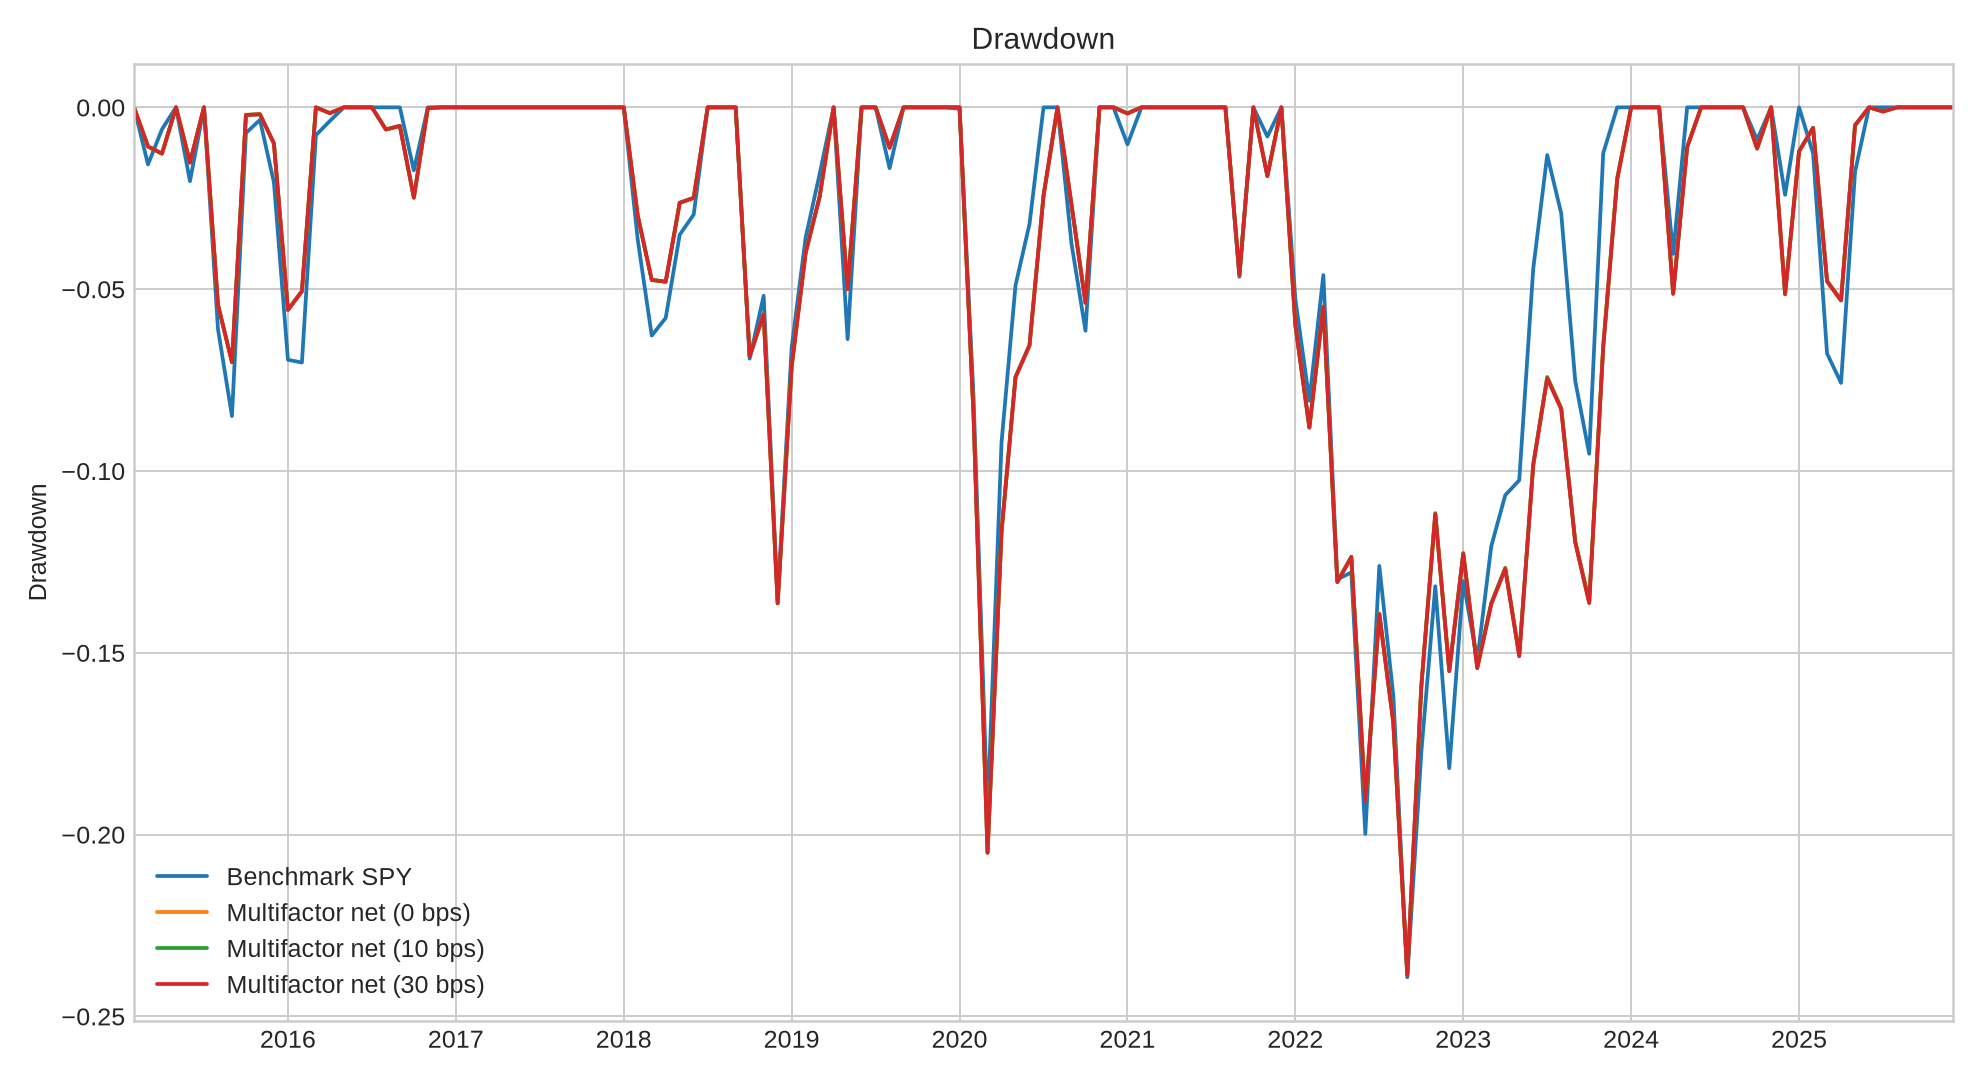
\includegraphics[width=0.92\linewidth,height=0.66\textheight,keepaspectratio]{assets/drawdown.png}
  \par\small\color{wcprimary}Drawdown maximal : $-23,85$\,\% à 10 pb contre $-23,93$\,\% pour SPY.
  \source{Figure du mémoire ; results/drawdowns.csv et results/metrics.csv.}
  \oral{Annexe. Utiliser si le jury interroge la protection en phase de baisse. Le maximum drawdown est mesuré sur les valeurs mensuelles et ne décrit pas les pertes intramensuelles. La différence entre les portefeuilles est très faible.}{latex/figures/drawdown.png ; results/drawdowns.csv ; results/metrics.csv ; backtest.py.}
\end{frame}

\begin{frame}{Annexe · Pourquoi le coût nul est accepté}
  \begin{itemize}\raggedright
    \item Coût réel du 31/12/2025 en fraction : $5{,}362\times10^{-6}$.
    \item Tolérance absolue du validateur : $10^{-4}$.
    \item L'écart avec zéro est inférieur à la tolérance.
  \end{itemize}
  \[
    |0-0{,}000005362| < 0{,}0001
  \]
  \takeaway{La précision attendue doit dépendre de l'échelle du champ.}
  \source{results/complementary\_analysis.json ; code du validateur.}
  \oral{Annexe. Les comparaisons portent sur des fractions, pas sur les pourcentages affichés. Une tolérance raisonnable pour un rendement peut être excessive pour un coût très faible. Préciser la convention d'arrondi et la précision propre à chaque champ.}{results/complementary\_analysis.json ; deepseek\_agent\_workflow.py ; evaluate\_deepseek.py.}
\end{frame}

\begin{frame}{Annexe · Sources et reproductibilité}
  \small
  \begin{itemize}\raggedright
    \item \textbf{Mémoire :} chapitres 3 à 6, protocole et analyse critique.
    \item \textbf{Finance :} \texttt{metrics.csv}, \texttt{period\_metrics.csv}.
    \item \textbf{Archive LLM :} \texttt{deepseek\_evaluation.json}.
    \item \textbf{Notes :} \texttt{note\_comparison.md}.
    \item \textbf{Contre-exemples :} \texttt{complementary\_analysis.json}.
  \end{itemize}
  \vspace{0.6em}
  \textbf{Rejouer l'analyse complémentaire, sans appel API :}\\[0.35em]
  \texttt{experience/.venv/bin/python analyze\_note\_comparison.py}
  \source{Fichiers du projet ; valeurs issues des résultats archivés.}
  \oral{Annexe. Montrer les artefacts pour inspecter les preuves. Les fichiers de résultats sont dans results/. Le script complémentaire conserve les transformations, les scores et les empreintes des sources. La note complète permet de dépasser les extraits montrés pendant l'oral.}{README.md ; analyze\_note\_comparison.py ; results/.}
\end{frame}
\end{document}
